\documentclass{article}

\usepackage[utf8]{inputenc}
\usepackage{csquotes}
\usepackage[english]{babel}
\usepackage[margin=1.2in]{geometry}
\usepackage{todonotes}
\usepackage{appendix}
\usepackage[final]{pdfpages}
\usepackage{amsmath}
\usepackage{hyperref}
\usepackage[capitalize]{cleveref}
\usepackage{utopia}
\usepackage{cite}
\usepackage{tikz}
\usepackage{caption}

\usepackage{amssymb} 
\usepackage{hyperref}
\usepackage{color}
%\usepackage{minted}
%\setminted{frame=lines}

\usepackage{subcaption}
\usepackage{graphicx} % Provides the \includegraphics command.
\usepackage{booktabs} % Better tables. Provides \toprule, \midrule, \bottomrule.
\usepackage{listings} % Provides source code listings.
\usepackage{todonotes} % Provides several handy TODO commands.
\usepackage{soul} % For striketrough

%\usepackage{subfig}
\usepackage{tabularx} %table config
\usepackage{colortbl} %table config
\usepackage{graphicx}%table config 
\usepackage{makecell}%table config
\usepackage{float}%table config

%%Code includes start
\usepackage{listings}
\usepackage{color}

\crefname{lstlisting}{listing}{listings}
\Crefname{lstlisting}{Listing}{Listings}

\definecolor{dkgreen}{rgb}{0,0.6,0}
\definecolor{gray}{rgb}{0.5,0.5,0.5}
\definecolor{mauve}{rgb}{0.58,0,0.82}

\lstset{frame=tb,
  language=Java,
  aboveskip=3mm,
  belowskip=3mm,
  showstringspaces=false,
  columns=flexible,
  basicstyle={\small\ttfamily},
  numbers=none,
  numberstyle=\tiny\color{gray},
  keywordstyle=\color{blue},
  commentstyle=\color{dkgreen},
  stringstyle=\color{mauve},
  breaklines=true,
  breakatwhitespace=true,
  tabsize=3,
}
%%Code includes end





\DeclareUnicodeCharacter{2212}{-} %google said I should include 
%% Front page
\renewcommand{\baselinestretch}{1.15} 

\AtBeginEnvironment{appendices}{\crefalias{section}{appendix}} %Fix cref appendix

\begin{document}
\begin{titlepage}
      \begin{center}
        \begin{figure}[h!]
            \centering
            \includegraphics[scale=0.2]{Figurer/ntnu.png}
            \label{fig:ntnu}
        \end{figure} 
        \vspace*{1cm}
        {\Large{TTK4550}}\\[0.4cm] 
        {\Large{\textit{Assessment of the exposure of publicly discoverable cyber-physical systems }}}\\[0.5cm]
        {\Huge{Report in progress}}\\[0.5cm] 
        {\Large{Sigurd Hellesvik}}\\[0.4cm] %%student numbers only, no names
        \large{\today}
        \vspace{1cm}
    \end{center}
    \vspace*{\fill}
\end{titlepage}


%% Table of contents
\thispagestyle{empty} % Avoid page numbering on the table of contents.
\linespread{1.15}
\newpage
\tableofcontents{}
\def\tableofcontentsname{test}
\thispagestyle{empty} % Avoid page numbering on the table of contents.


%%% Main content %%%
%\newpage
\setcounter{page}{1}
\todo{see \cref{sec:new} to find new stuff}

\section{Introduction} \label{sec:intro}
While a lot of the Cyber-Physical Systems(CPS) connected to the internet are well maintained and secure, many other are vulnerable. This is most often because the CPSs are not set up properly or run outdated software. Other than this, it is a "fact" of statistics that if a quantity CPSs are connected to the internet, a portion of these will be insecure. To explore the extent of this challenge, the first step is to identiy how many CPSs can be reached. The search engine \href{https://shodan.io}{\color{blue}{Shodan}} is a popular search engine for enumerating Internet-connected systems. Because of the sheer number of  publicly accessible devices, not all can be mapped here, and constraints have to be set. These constraints decide a focus on CPS belonging to the European maritime and offshore industries.

\subsection{Collaboration}\label{sec:collaboration}
This project is a collaboration between the main supervisor Mary Ann Lundteigen and PhD candidate Bálint Zoltán Téglásy, both representing NTNU; and the Global Service Line Leade, Cybersecurity, at DNV-GL Trondheim,  Mate J Csorba. The student carrying out the project is Sigurd Hellesvik.

\subsubsection{DNV-GL}\label{sec:dnvgl}
DNV-GL are a independent expert in risk management and quality assurance. The abbreviation is for "Det Norske Veritas" and "Germanischer Lloyd". A big portion of their focus is on the maritime and offshore business. The DNV-GL has a Cyber Security team that helps customers assess and manage risks related to cyber security.~\cite{DNVGL_cybersec}  The International Maritime Organisation (IMO) "encourages administrations to ensure that cyber risks are appropriately addressed in existing safety management systems (as defined in the ISM Code) no later than [...] 1 January 2021".~\cite{IMO_2021} Because of this, many maritime cooperations will have to pay more attention to cyber security; making maritime cyber security specialists like DNV-GL Cyber Security team all the more revelant for the business. 

\subsection{Project goal}\label{sec:goal}
\textbf{The goal of this project is to map of Cyber-Physical Systems(CPS) in the European maritime and offshore industry that is reachable trough the internet, and by doing so get an overview of the exposure of these cyber-physical systems.}




\section{Project description} \label{sec:desc}

\subsection{Cyber-Physical Systems(CPS)}\label{sec:cps}
Cyber-Physical Systems(CPS) can be defined as "engineered systems that integrate information technologies, real‐time control subsystems, physical components, and human operators to influence physical processes by means of cooperative and (semi)automated control functions."~\cite{guzman_wied_kozine_lundteigen_2019}
CPS is a broad term, and examples can be everything automated control systems at offshore platforms to the computer system in an electric car. As more and more of the CPSs are connected to the internet, cyber threats becomes a bigger challenge. 

\subsection{Search engine} \label{sec:shodan_intro}
Shodan is a search engine like Google. Instead of searching for web pages, however, it will gather publicly-available information about all devices directly connected to the internet.~\cite{shodan} This makes Shodan ideal for mapping all CPSs that are connected to the internet. 
Earlier in this pre-report, the search engine Shodan has been assumed used. This is not the only alternative, as other tools like \href{https://censys.io/}{\color{blue}{Censys}} and \href{www.zoomeye.org}{\color{blue}{ZoomEye}} have functionality similar to Shodan. It is, however, enough to use one of the engines. Shodan is chosen, since it is arguably the most popular choice, and therefore, more documentation and examples can be found. Another assessment of this choice can be made later, if found necessary. 

\subsection{Constraints}\label{sec:constraints}
Shodan will list a lot of different IP addresses and info about them. This will be to much for this project, so constraints have to be set. The factors that will decide the constraints will be Competence, Info Available and Relevance. While this type of project normally is reserved for Computer Science students, Sigurd is studying Cybernetics and Robotics. This could for example make meaningful to focus on industrial CPSs. In addition, the competence of the supervisors should be taken into accord. Mary Ann has worked Offshore, Mate has experience with cruise ships and Bálint work with power plants. This project will therefore focus on the Maritime and Offshore industries. With this constraints, too many results might still be present. To narrow the results some more, a reginal constraint will be set. Only CPSs in Europa will be concidered. Depending on how different CPS are implemented, different information might be available on Shodan. To get useful results, constraints will probably be set based on hardware and/or protocols. Research and testing will have to be done before these constraints eventually have to be set. The constraints may generally be changed later in the project, if the results prove to be too few or too many.

\subsection{Project work}\label{sec:work} \todo{This is a part of the previous plan, and should be chenged soon}
After the initial planning is done, the project work can begin. First, scripts will be written that use the Shodan API to gather data based on the constraints. Then different tools will be utilized to sort the information, and make it presentable. This could for example be heat maps to show geographic, graphs to compare results or infographics. If there is more time after this is done, the student might look into the actual security of the CPS mapped. To quote a suggestion from Mate: "This can include manual probing, targeted vulnerability scan of resulting IPs with OpenVAS". In that case, the student will first have to learn the techniques, then perform the testing.
\newpage

\section{Tentative plan}\label{sec:plan}
 Sigurd will meet with Bálint once a week to discuss progress. Mate will be invited to these meetings, and sent a protocol afterwards. Sigurd will meet with Mary Ann every odd week. There is not yet any set time for these meetings. \\
In the table, the individual tasks are planned finished before the corresponding date, which is always Thursdays. This means that work on the next step begins on Thursdays.
\newline


\begin{tabular}{|l|l|l|}
\hline
Week & Date & Tentative plan                                                                     \\ \hline
Week 35 & 27.08.2020 & First draft pre-study report                                              \\ \hline
Week 36 & 03.09.2020 & Finish pre-study report + research, aka find at least 3 relevant sources  \\ \hline
Week 37 & 10.09.2020 & Research(3 sources)                                                       \\ \hline
Week 38 & 17.09.2020 & Get to know Shodan, also API                                              \\ \hline
Week 39 & 24.09.2020 & Testing different constraints                                             \\ \hline
Week 40 & 01.10.2020 & Deadline for deciding constraints                                         \\ \hline
Week 41 & 08.10.2020 & Work on project                                                           \\ \hline
Week 42 & 15.10.2020 & Investigate HTML5 and make figures                                        \\ \hline
Week 43 & 22.10.2020 & Investigate traceroute                                                    \\ \hline
Week 44 & 29.10.2020 & Write results for the different methods                                   \\ \hline
Week 45 & 05.11.2020 & Meeting DNVGL + Look into sugestions by DNVGL                                             \\ \hline
Week 46 & 12.11.2020 & Full plan for report                                                      \\ \hline
Week 47 & 19.11.2020 & Finish first draft report + get feedback                                  \\ \hline
Week 48 & 26.11.2020 & Exams                                                                     \\ \hline
Week 49 & 03.12.2020 & Exams                                                                     \\ \hline
Week 50 & 10.12.2020 & Finishing touches + make presentation                                     \\ \hline
Week 51 & 17.12.2020 & Deadline                                                                  \\ \hline
\end{tabular}


\section{Literature} \label{sec:literature}
\subsection{Articles} \label{sec:articles}
\subsubsection{Cybersecurity and Safety Co-Engineering of Cyberphysical systems -A Comprehensive Survey}
This article look into how recent methods to implement cybersecurity and Safety in CPS. Safety and cybersecurity are often interconnected, and affect the same systems. While they often are complemnentary, other times safety and cybersecurity are in conflict. The aricle in question use a good example, where a door will open on power loss to ensure the safety of workers. However, cybersecurity want the same door to close on power loss, to stop intruders. The article look at a sample of studies on the subject from the last 20 years, and compares them. The conclusion is to see what topics need more research. How can this be relevant for the report?

\subsubsection{Shodan Vizualized}
The article \textit{Shodan Visualized} gives a map of SCADA devices connected to the internet.\cite{ercolani_patton_chen_2016} This is good to prove the point that a lot of CPSs are connected. For myself: Look into difference between CPS and SCADA. 

\subsubsection{Evaluation of the ability of the Shodan search engine to identify Internet-facing industrial control devices}
\textit{Evaluation of the ability of the Shodan search engine to identify Internet-facing industrial control devices} gives a good overview of how Shodan works, with an explanation of the Shodan process for indexing webpages.\cite{bodenheim_butts_dunlap_mullins_2014} 
In addition, it shows how Shodan can be used to search for Industrial Control Devices(ICS). A lot of those ICS will be used in the offshore industry, and some in the maritime industry. 
Lastly, the report shows that obfuscating devices make them harder to find using Shodan.

\subsection{Standards} \label{sec:standards}
\subsubsection{IEC 62443} \label{sec:IEC62443}
The IEC 62443 series is a series of technical reports and standards that defines procedures for how to implement secure Industrial Automation and Control Systems (IACS), focusing on the cybersecurity of these systems. This series covers multiple industries.

\subsubsection{DNVGL-RP-G108} \label{sec:G108}
Due to the scope of IEC 62443 being general, it can be time consuming to implement it for different standards.
For the Oil and Gas sector, the DNVGL-RP-G108 is a recommended practice for implementing IEC 62443. While the implementation of cybersecurity functions are not relevant to for mapping CPS, it can be useful to know more about the different systems that can be exposed to the internet. In that way, it can be discussed which procedures of the DNVGL-RP-G108 are used to secure IACS against eventual threats coming trough internet connections.

\subsection{Shodan}\label{sec:shodan}
Shodan is a search engine like Google. Instead of searching for web pages, however, it will gather publicly-available information about all devices directly connected to the internet.~\cite{shodan} This makes Shodan ideal for mapping all CPSs that are connected to the internet.

\subsubsection{Shodan account}
It is possible to make up to 5 queries using Shodan without registering an account. 
With a free account, it is possible to perform more queries, access the Shodan API, and get limited access to search filters. However, without a paid account, the search engine has limitations.
Using the API, a free user can access up to 100 results from searches. 
For paid users, there are three payment plans: Freelancer, Small Business and Corporate. A Freelancer user gets access to up to 1 million results per month and access to most search filters. 
Users paying for the higher tiers can get from 20 million to an unlimited number of results, all search filters and multiple extra benefits. 
The Freelancer payment plan will be sufficient for the scope of this project.

\subsubsection{Crawlers and banners}
Shodan has bots called "crawlers" to find information about devices connected to the internet, such as IP address, port number, country, service running, version, protocols used, and more. 
All these properties are saved in Shodan "banners" . The creator of Shodan, John Matherly has described banners as "A banner is simply metadata about a service.". \cite{banner} 
Therefore, when a user starts a search using the Shodan search engine, it will not return live results, but rather the banners already saved in the Shodan database. Shodan guarantees that returned banners have been collected in the last 30 days.\cite{matherly_guide_to_shodan}
Some of the Shodan banner properties are always on banners, while others are situational. For example will SSL properties only occur on banners of ports that use SSL encryption. A complete list of both required and situational Shodan banner properties can be found in \cref{app:banner_properties}.
Normally, the banners are in the JSON format. An example of a banner can be found in \cref{app:marlink_banner}.
Matherly\cite{matherly_guide_to_shodan} describes the basic algorithm for Shodan crawlers as:
\begin{enumerate}
\setlength\itemsep{0em}
	\item Generate a random IPv4 address. 
	\item Generate a random port to test from the list of ports that Shodan understands.
	\item Check the random IPv4 address on the random port and grab a banner.
	\item Goto 1
\end{enumerate}
The list of ports mentioned can be found by using the API web call in \cref{lst:api_ports}.

\subsubsection{Search filters} \label{sec:filters}
To limit the results returned from a Shodan query, filters are applied. Filters are on the format:
\begin{lstlisting}
filter_property: value
\end{lstlisting}
When using a filter, Shodan queries will return banners where the properties specified in the filter contain the specified value. In most cases, filter properties correspond with banners. However, some filter properties are not banner properties. For example the "geo" filter property can define an area. The Shodan query will then return all banners where the "location.latitude" and "location.longitude" properties are within this area. 

A comprehensive list of the Shodan filters can be found in \cref{app:shodan_filters}, . The queries used in this project will be explained in more detail. 

\subsection{Previous research}
Since Shodan was launched in 2009, a lot of research has been done in order to finding ICS using Shodan. The Shodan website even has its own article on the subject.\cite{shodan_ics} There also exist other lists of Shodan queries that will find ICS systems. For example, the website SCADA Strangelove has compiled multiple such lists, focusing on both Supervisory Control And Data Acquisition (SCADA) and ICS devices.\cite{scadasl_cheatsheet} \cite{scadasl_shodan}

On the other hand, research exist on ICS defense against Shodan scans. For example, \textit{Evaluation of the ability of the Shodan search engine to identify Internet-facing industrial control devices} by Bodenheim, Butts, Dunlap and Mullins, \cite{bodenheim_butts_dunlap_mullins_2014} demonstrates how obfuscation can be used to mask ICS devices from Shodan searches. Furthermore, the article implemented this on several honeypots. A honeypot is a computer that is configured to look like another device, in this case an ICS. Then the honeypot will log all traffic. Bodenheim, Butts, Dunlap and Mullins had an independent researcher try to find the devices using Shodan, showing how the devices were harder to find when obfuscated.

\newpage




\section{Search Terms Shodan} \label{sec:search_term}
This list is temporary, and more to remember past searches than to actually use in a final report.
\begin{table}[H]
\centering
\begin{tabular}{|l|l|l|}
\hline
Search term & Hits & Found \\ \hline
inmarsat & 7 & From \cite{maritime_pen_test} \\ \hline
Sailor 900 & 3 & From \cite{maritime_pen_test} \\ \hline
Sailor & 32 & From \cite{maritime_pen_test} \\ \hline
thrane & 5 & From \cite{maritime_pen_test} \\ \hline
marlink & 32 &  From thrane search, keywork on one of hits \\ \hline
sealink & 4 &  from marlink website\\ \hline
xchange & 82 &  from marlink website. Possibly name used for different things\\ \hline
navtex & 2 &  from \cite{maritime_digitalization}\\ \hline
nbdp & 3 &  from \cite{maritime_digitalization}\\ \hline
gmdss & 16 &  from \cite{maritime_digitalization}\\ \hline
AIS & 2876 &  from \cite{maritime_digitalization}\\ \hline
furuno & 5 &  from \cite{maritime_digitalization}\\ \hline
LRIT & 12 &  from \cite{maritime_digitalization}\\ \hline
radar & 734 &  a lot of ships have radar right?\\ \hline
MArine Stabilized Antenna System & 23 &  "Hacking Yatch remotely" PowerPoint\\ \hline
E2500 & 774 &  Maretrons nettside\\ \hline
isp:tampnet & 95 &  tampnet is a internet provider for offshore systems\\ \hline
net:185.96.40.0/23 & 23 &  used https://api.hackertarget.com/aslookup/?q=185.96.41.27\\ \hline
net:185.96.40.0/23 & 30 &  same as previous, but using ZoomEye\\ \hline

port:10110 & 4 &  List of TCP and UDP ports, NMEA\\ \hline
NMEA & 67 &  NMEA is a maritime communication protocol\\ \hline


search & hits &  found\\ \hline
\end{tabular}
\end{table}


%%https://en.wikipedia.org/wiki/NMEA_2000_PGN
\section{Theory}

\subsection{IPv4}
To navigate the internet, the IP protocol is used. This is mainly split into the popular IPv4 and the new IPv6. IPv4 addresses are 32 bit, meaning they can range from 0.0.0.0 to 255.255.255.255. 

\subsubsection{IPv6}
The solution to the exhaustion of IPv4 address space is IPv6. This protocol has $2^{128}$ unique addresses, so it will be able to cover the forseable future. The global conversion from IPv4 to IPv6 is slow, however.While Shodan does support IPv6, most corporations in the maritime and offshore industries are big enough to have, and use, IPv4 addresses. 


\subsection{IP range}
 The IPv4 addresses are sold to organisations, for them to distribute further. For example, an Internet Service Provider (ISP) like Telenor will give IPv4 addresses to the customers while they use their subscribed internet connections. This distribution of IPv4 addresses to organisations is illustrated in \cref{fig:ipv4_map}.

\begin{figure}
    \centering
    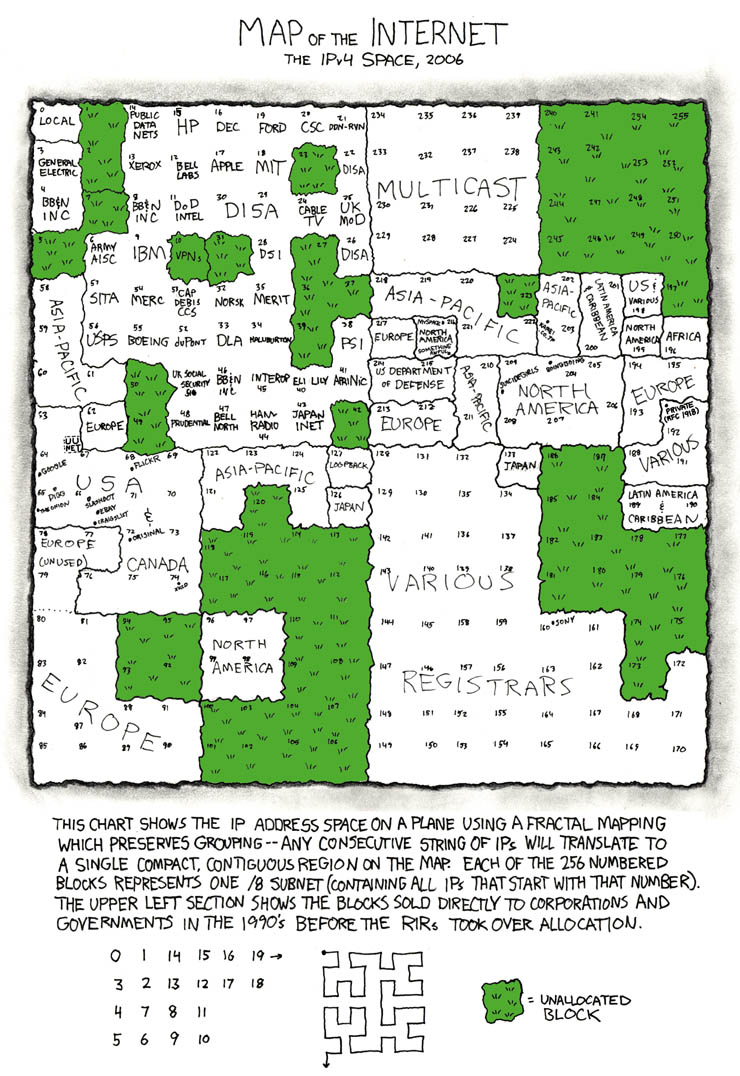
\includegraphics[scale=4]{Figurer/map_of_the_internet.jpg}
    \caption{A map of the IPv4 space, from the XKCD webcomic. \cite{xkcd} }
    \label{fig:ipv4_map}
\end{figure}

\subsubsection{IPv4 exhaustion and NAT}
IPv4 addresses were distributed by the Internet Assigned Numbers Authority (IANA). 11 January, 2011, IANA allocated its last block.\cite{exhasuted_IPV4} Since then, the regional bodies responsible for allocationg IPv4 addresses, Regional Internet Registries (RIR), have also exhausted their IPv4 addresses, the last one in 2019.\cite{exhausted_RIPENNC} Due to this problem, multiple methods are used to get the most out of the IPv4 address space. Arguably, the most popular of these methods are Network Address Translation (NAT).

NAT lets you connect multiple devices to the same IPv4. This is done by using a routing device with a shared IPv4 address to receive packages for multiple different devices, and then redirect the packages to the correct receiver. This makes it so that the devices behind the NAT can reach the internet, while communication from the internet can not reach the devices unless the devices start the communication. This connection is illustrated in \cref{fig:NAT} 

\tikzset{every picture/.style={line width=0.75pt}} %set default line width to 0.75pt        
\begin{tabular}{p{10cm}}
   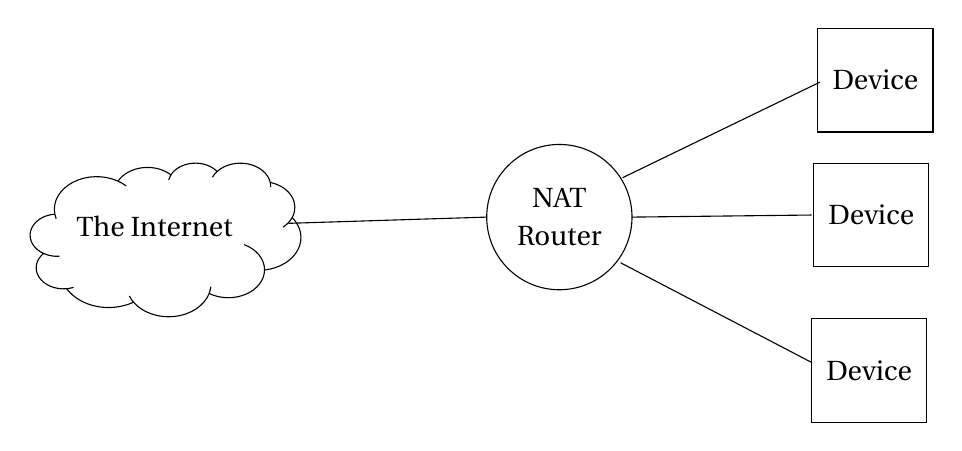
\begin{tikzpicture}[x=0.75pt,y=0.75pt,yscale=-1,xscale=1]
     %uncomment if require: \path (0,300); %set diagram left start at 0, and has height of 300

%Shape: Rectangle [id:dp7550808737565868] 
\draw   (417.5,74) -- (473,74) -- (473,124) -- (417.5,124) -- cycle ;

%Shape: Ellipse [id:dp5744265006375734] 
\draw   (258,165) .. controls (258,145.67) and (273.67,130) .. (293,130) .. controls (312.33,130) and (328,145.67) .. (328,165) .. controls (328,184.33) and (312.33,200) .. (293,200) .. controls (273.67,200) and (258,184.33) .. (258,165) -- cycle ;

%Straight Lines [id:da011152119100300673] 
\draw    (418.5,100) -- (323.5,146) ;
%Shape: Rectangle [id:dp019726233695570805] 
\draw   (414.5,214) -- (470,214) -- (470,264) -- (414.5,264) -- cycle ;

%Shape: Rectangle [id:dp2854982925574172] 
\draw   (415.5,139) -- (471,139) -- (471,189) -- (415.5,189) -- cycle ;

%Straight Lines [id:da042657718924057675] 
\draw    (414.5,164) -- (328,165) ;
%Straight Lines [id:da8590380439733557] 
\draw    (414.5,235) -- (322.5,187) ;
%Shape: Cloud [id:dp5209862047408297] 
\draw   (49.88,163.36) .. controls (48.82,157.4) and (52.27,151.49) .. (58.76,148.15) .. controls (65.25,144.81) and (73.64,144.62) .. (80.36,147.67) .. controls (82.74,144.2) and (87.1,141.8) .. (92.13,141.21) .. controls (97.15,140.61) and (102.24,141.88) .. (105.86,144.64) .. controls (107.89,141.49) and (111.87,139.38) .. (116.4,139.05) .. controls (120.93,138.71) and (125.35,140.21) .. (128.11,143.01) .. controls (131.78,139.67) and (137.61,138.27) .. (143.09,139.4) .. controls (148.57,140.54) and (152.7,144) .. (153.71,148.31) .. controls (158.2,149.25) and (161.95,151.66) .. (163.97,154.91) .. controls (166,158.15) and (166.1,161.92) .. (164.27,165.23) .. controls (168.7,169.68) and (169.73,175.61) .. (166.99,180.8) .. controls (164.25,186) and (158.14,189.68) .. (150.95,190.48) .. controls (150.9,195.35) and (147.44,199.83) .. (141.9,202.17) .. controls (136.37,204.52) and (129.62,204.38) .. (124.26,201.79) .. controls (121.98,207.63) and (115.55,211.93) .. (107.76,212.83) .. controls (99.97,213.73) and (92.21,211.06) .. (87.83,205.99) .. controls (82.46,208.49) and (76.02,209.21) .. (69.96,207.99) .. controls (63.9,206.77) and (58.74,203.7) .. (55.62,199.49) .. controls (50.14,199.99) and (44.84,197.79) .. (42.35,194) .. controls (39.86,190.2) and (40.71,185.61) .. (44.49,182.5) .. controls (39.59,180.28) and (37.1,175.87) .. (38.3,171.56) .. controls (39.5,167.26) and (44.13,164.05) .. (49.76,163.59) ; \draw   (44.49,182.5) .. controls (46.8,183.55) and (49.46,184.03) .. (52.13,183.87)(55.62,199.49) .. controls (56.77,199.39) and (57.89,199.17) .. (58.97,198.84)(87.83,205.99) .. controls (87.02,205.06) and (86.34,204.06) .. (85.81,203.01)(124.26,201.79) .. controls (124.67,200.73) and (124.95,199.63) .. (125.06,198.52)(150.95,190.48) .. controls (151.01,185.28) and (147.19,180.53) .. (141.14,178.26)(164.27,165.23) .. controls (163.29,167) and (161.79,168.57) .. (159.9,169.81)(153.71,148.31) .. controls (153.88,149.02) and (153.95,149.75) .. (153.94,150.47)(128.11,143.01) .. controls (127.2,143.84) and (126.44,144.77) .. (125.87,145.77)(105.86,144.64) .. controls (105.37,145.39) and (105.01,146.19) .. (104.77,147.02)(80.36,147.67) .. controls (81.78,148.31) and (83.1,149.09) .. (84.28,149.97)(49.88,163.36) .. controls (50.02,164.19) and (50.25,165) .. (50.56,165.79) ;

%Straight Lines [id:da9624009852798121] 
\draw    (162.5,168) -- (258,165) ;

% Text Node
\draw (293,165) node   [align=left] {\begin{minipage}[lt]{33.354pt}\setlength\topsep{0pt}
\begin{center}
NAT\\Router
\end{center}

\end{minipage}};
% Text Node
\draw (445.25,99) node   [align=left] {Device};
% Text Node
\draw (442.25,239) node   [align=left] {Device};
% Text Node
\draw (443.25,164) node   [align=left] {Device};
% Text Node
\draw (59,163) node [anchor=north west][inner sep=0.75pt]   [align=left] {The Internet};

   \end{tikzpicture}
   \captionof{figure}{Illustration of a NAT router}
   \label{fig:NAT}
\end{tabular}


\subsubsection{CIDR}
 Classless Inter-Domain Routing(CIDR) is the modern way to split the IPv4 address space into blocks, so that they can be distributed. A CIDR block can look like this: "93.192.0.0/10". This block has two parts, the prefix "93.192.0.0" and the suffix "/10". The prefix indicates the size of the CIDR block. The prefix indicates where in the IPv4 space the CIDR block is located. To understand this, it is useful to look at an IP address in binary instead of decimal. For example, the IPv4 address "93.220.107.30" becomes "01011101.11011100.01101011.00011110". The suffix decides how many bits are fixed. In the CIDR block "93.220.107.30/10", the 10 first bits of the prefix "93.220.107.30"  are "01011101.11xxxxxx.xxxxxxxx.xxxxxxxx". This number span the binary range \\ \{01011101.11111111.11111111.11111111 - 01011101.11000000.00000000.00000000 \}, or the decimal range  \{ 93.192.0.1 - 93.255.255.254 \}. Remark that not the full prefix is needed; "93.220.107.30/10" and "93.220.107.31/10" are the same CIDR  block. Because of this, it is normal to set the changing bits of the prefix to 0, as in: "93.192.0.0/10". 
Since the sizes of CIDR blocks vary, they can be nested. For example, "93.192.0.0/11" is a part of "93.192.0.0/10".


\section{WORK IN PROGRESS} \label{sec:new}












%% Appendix
\newpage
\begin{appendices} \label{appendix}
\input{"appendix/dictionary"}
\input{"appendix/project_announcement"}
\section{API commands}
Commands used for interacting with the Shodan API. Both using the Shodan REST APi directly \cite{api_ref} and the Shodan Python Command Line Interface(CLI)\cite{cli_ref}.

\begin{lstlisting}[label=lst:api_ports,caption=Ports web API call]
https://api.shodan.io/shodan/ports/?key={YOUR_API_KEY}
\end{lstlisting}
\input{"appendix/search_filters"}
\input{"appendix/banner_example"}
\end{appendices}


%% References
\newpage
\bibliography{references}{}
\bibliographystyle{plain}



\end{document}
